\begin{answer}
It is possible to have a set of weights that allow the neural network to classify this dataset with 100\% accuracy
\begin{figure}[htbp] 
	\centering
	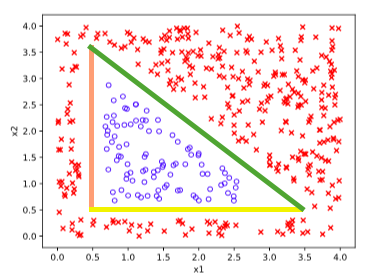
\includegraphics[scale=0.7]{tex/01-simple_nn/1(b)step_function.png}
	\caption{contour of the two classes}
\end{figure}\\
It's obvious to see that the class 0's contour is a triangle. The three  vertices of the triangle is $(0.5, 0.5), (0.5, 3.5), (3.5, 0.5)$. The points of the class 0 should above the yellow line, on the right of the red line and under the green line. Thus, we can get three inequalities(the horizontal line is $x_1$, the vertical one is $x_2$):
\begin{align*}
    &x_1 - 0.5 \geq 0\\
    &x_2 - 0.5 \geq 0\\
    &x_1 + x_2 - 4 \leq 0
\end{align*}
So, the $w^{[1]}$ matrix (the $j$ th row $i$ th col item is $w^{[1]}_{i - 1, j}$ should be $$\begin{bmatrix}-0.5 & 1 & 0\\ -0.5 &  0 & 1\\
-4 & 1 & 1\end{bmatrix}$$
Also, the hidden state for the class 0 is $h = \begin{bmatrix}  1\\ 1\\ 0\end{bmatrix}$. We need to design a $w^{[2]}$ that can distinguish $\begin{bmatrix}1 \\ 1 \\ 0\end{bmatrix}$ with other seven possible states. $w^{[2]} = \begin{bmatrix}10 \\ -6 \\ -6 \\ 10^{10}\end{bmatrix}$ is a valid choice.
\end{answer}
